\documentclass[a4paper]{jpconf}
\usepackage{graphicx}
\usepackage{./definitions}
\usepackage{lineno,hyperref}
\usepackage{amsmath}
\usepackage{amsfonts}
\usepackage{amssymb}
\usepackage{amsthm}
\usepackage{mathrsfs}
\usepackage{color}
\usepackage{url}
\usepackage[numbers]{natbib}

\newcommand{\ee}[1]{{\color{red} EE:~#1}}
\newcommand{\rc}[1]{{\color{blue} RC:~#1}}
\newcommand{\modified}[1]{{\color{red} #1}}

\bibliographystyle{iopart-num}

\begin{document}
\title{\texttt{thornado}-transport: IMEX schemes for two-moment neutrino transport respecting Fermi-Dirac statistics}

\author{Ran Chu}
\address{Department of Physics and Astronomy, University of Tennessee, Knoxville, TN 37996-1200}
\ead{rchu@vols.utk.edu}

\author{Eirik Endeve}
\address{Computational and Applied Mathematics Group, Oak Ridge National Laboratory, Oak Ridge, TN 37831 USA}
\address{Department of Physics and Astronomy, University of Tennessee, Knoxville, TN 37996-1200}
\address{Joint Institute for Computational Sciences, Oak Ridge National Laboratory, Oak Ridge, TN 37831 USA}
\ead{endevee@ornl.gov}

\author{Cory D. Hauck}
\address{Computational and Applied Mathematics Group, Oak Ridge National Laboratory, Oak Ridge, TN 37831 USA}
\address{Department of Mathematics, University of Tennessee, Knoxville, TN 37996-1320}
\ead{hauckc@ornl.gov}

\author{Anthony Mezzacappa}
\address{Department of Physics and Astronomy, University of Tennessee, Knoxville, TN 37996-1200}
\address{Joint Institute for Computational Sciences, Oak Ridge National Laboratory, Oak Ridge, TN 37831 USA}
\ead{mezz@utk.edu}

\author{Bronson Messer}
\address{Scientific Computing and Theoretical Physics Groups, Oak Ridge National Laboratory, Oak Ridge, TN 37831 USA}
\address{Department of Physics and Astronomy, University of Tennessee, Knoxville, TN 37996-1200}
\ead{bronson@ornl.gov}

\begin{abstract}
We develop implicit-explicit (IMEX) schemes for neutrino transport in a background material in the context of a two-moment model that evolves the angular moments of a neutrino phase-space distribution function.
Considering the upper and lower bounds that are introduced by Pauli's exclusion principle on the moments, an algebraic moment closure based on Fermi-Dirac statistics and a convex-invariant time integrator both are demanded.
A finite-volume/first-order discontinuous Galerkin(DG) method is used to illustrate how an algebraic moment closure based on Fermi-Dirac statistics is needed to satisfy the bounds.
Several algebraic closures are compared with these bounds in mind, and the Cernohorsky and Bludman closure, which satisfies the bounds, is chosen for our IMEX schemes.
For the convex-invariant time integrator, two IMEX schemes named PD-ARS have been proposed.
PD-ARS denotes a convex-invariant IMEX Runge-Kutta scheme that is high-order accurate in the streaming limit, and works well in the diffusion limit.
Our two PD-ARS schemes use second- and third-order, explicit, strong-stability-preserving Runge-Kutta methods as their explicit part, respectively, and therefore are second- and third-order accurate in the streaming limit, respectively.
The accuracy and convex-invariance of our PD-ARS schemes are demonstrated in the numerical tests with a third-order DG method for spatial discretization and a simple Lax-Friedrichs flux.
The method has been implemented in our high-order neutrino-radiation hydrodynamics (\texttt{thornado}) toolkit.
We show preliminary results employing tabulated neutrino opacities.
\end{abstract}

\section{Introduction}
\label{sec:intro}

In this paper we design numerical methods to solve a two-moment model that governs the transport of particles obeying Fermi-Dirac statistics (e.g., neutrinos), with the ultimate target being nuclear astrophysics applications (e.g., neutrino transport in core-collapse supernovae and compact binary mergers).  
The numerical method is based on the discontinuous Galerkin (DG) method for spatial discretization and implicit-explicit (IMEX) methods for time integration, and it is designed to preserve certain physical constraints of the underlying model.  
The latter property is achieved by considering the spatial and temporal discretization together with the closure procedure for the two-moment model.  

In many applications, the particle mean free path is comparable to or exceeds other characteristic length scales in the system under consideration, and non-equilibrium effects may become important.  
In these situations, a kinetic description based on a particle distribution function may be required.  
The distribution function, a phase space density $f$ depending on momentum $\vect{p}\in\bbR^{3}$ and position $\vect{x}\in\bbR^{3}$, is defined such that $f(\vect{p},\vect{x},t)$ gives at time $t\in\bbR^{+}$ the number of particles in the phase space volume element $d\vect{p}\,d\vect{x}$ (i.e., $d\cN=f\,d\vect{p}\,d\vect{x}$).  
The evolution of the distribution function is governed by the Boltzmann equation, which states a balance between phase space advection and particle collisions (see, e.g., \cite{braginskii_1965,chapmanCowling_1970,lifshitzPitaevskii_1981}).  

Solving the Boltzmann equation numerically for $f$ is challenging, in part due to the high dimensionality of phase space.  
To reduce the dimensionality of the problem and make it more computationally tractable, one may instead solve (approximately) for a finite number of angular moments $\vect{m}_{N}=(m^{(0)},m^{(1)},\ldots,m^{(N)})^{T}$ of the distribution function, defined as
\begin{equation}
  m^{(k)}(\varepsilon,\vect{x},t)=\f{1}{4\pi}\int_{\bbS^{2}}f(\omega,\varepsilon,\vect{x},t)\,g^{(k)}(\omega)\,d\omega,
\end{equation}
where $\varepsilon=|\vect{p}|$ is the particle energy, $\omega$ is a point on the unit sphere $\bbS^{2}$ indicating the particle propagation direction, and $g^{(k)}$ are momentum space angular weighing functions.  
In problems where collisions are sufficiently frequent, solving a \emph{truncated moment problem} can provide significant reductions in computational cost since only a few moments are needed to represent the solution accurately.  
On the other hand, in problems where collisions do not sufficiently isotropize the distribution function, more moments may be needed.  
In the two-moment model considered here ($N=1$), angular moments representing the particle density and flux (or energy density and momentum) are solved for.  
Two-moment models for relativistic systems appropriate for nuclear astrophysics applications have been discussed in, e.g., \cite{lindquist_1966,andersonSpiegel_1972,thorne_1981,shibata_etal_2011,cardall_etal_2013a}.  
However, in this paper, for simplicity (and clarity), we consider a non-relativistic model, leaving extensions to relativistic systems for future work.  

In a truncated moment model, the equation governing the evolution of the \mbox{$N$-th} moment $m^{(N)}$ contains higher moments $\{m^{(k)}\}_{k=N+1}^{M}$ ($M>N$), which must be specified in order to form a closed system of equations.  
For the two-moment model, the symmetric rank-two Eddington tensor (proportional to the pressure tensor) must be specified.  
Approaches to this \emph{closure problem} include setting $m^{(k)}=0$, for $k>N$ ($P_N$ equations \cite{brunnerHolloway_2005} and filtered versions thereof \cite{mcclarrenHauck_2010,laboure_etal_2016}), Eddington approximation (when $N=0$) \cite{mihalasMihalas_1999}, Kershaw-type closure \cite{kershaw_1976}, and maximum entropy closure \cite{minerbo_1978,cernohorskyBludman_1994,olbrant_etal_2013}.  
The closure procedure often results in a system of nonlinear hyperbolic conservation laws, which can be solved using suitable numerical methods (e.g., \cite{leveque_1992}).  

One challenge in solving the closure problem is constructing a sequence of moments that are consistent with a positive distribution function, which typically implies algebraic constraints on the moments \cite{kershaw_1976,levermore_1984}.  
Moments satisfying these constraints are called \emph{realizable moments} (e.g., \cite{levermore_1996}).  
When evolving a truncated moment model numerically, maintaining realizable moments is challenging, but necessary in order to ensure the well-posedness of the closure procedure \cite{levermore_1996,junk_1998,hauck_2008}.  
In addition to putting the validity of the numerical results into question, failure to maintain moment realizability in a numerical model may, in order to continue a simulation, require ad hoc post-processing steps with undesirable consequences such as loss of conservation.  

Here we consider a two-moment model for particles governed by Fermi-Dirac statistics.  
It is well known from the two-moment model for particles governed by Maxwell-Boltzmann statistics (``classical'' particles with $f\ge0$), that the particle density is nonnegative and the magnitude of the flux vector is bounded by the particle density.  
(There are further constraints on the components of the Eddington tensor \cite{levermore_1984}.)  
Furthermore, the set of realizable moments generated by the particle density and flux vector constitutes a convex cone \cite{olbrant_etal_2012}.  
In the fermionic case, there is also an upper bound on the distribution function (e.g., $f\le1$) because Pauli's exclusion principle prevents particles from occupying the same microscopic state.  
The fermionic two-moment model has recently been studied theoretically in the context of maximum entropy closures \cite{lareckiBanach_2011,banachLarecki_2013,banachLarecki_2017b} and Kershaw-type closures \cite{banachLarecki_2017a}.  
Because of the upper bound on the distribution function, the algebraic constraints on realizable moments differ from the classical case with no upper bound, and can lead to significantly different dynamics when the occupancy is high (i.e., when $f$ is close to its upper bound).  
In the fermionic case, the set of realizable moments generated by the particle density and flux vector is also convex. 
It is ``eye-shaped'' (as will be shown later; cf. Figure~\ref{fig:RealizableSetFermionic} in Section~\ref{sec:realizability}) and tangent to the classical realizability cone on the end representing low occupancy, but is much more restricted for high occupancy.  

In this paper, the two-moment model is discretized in space using high-order Discontinuous Galerkin (DG) methods (e.g., \cite{cockburnShu_2001,hesthavenWarburton_2008}).  
DG methods combine elements from both spectral and finite volume methods and are an attractive option for solving hyperbolic partial differential equations (PDEs).  
They achieve high-order accuracy on a compact stencil; i.e., data is only communicated with nearest neighbors, regardless of the formal order of accuracy, which can lead to a high computation to communication ratio, and favorable parallel scalability on heterogeneous architectures has been demonstrated \cite{klockner_etal_2009}.  
Furthermore, they can easily be applied to problems involving curvilinear coordinates (e.g., beneficial in numerical relativity \cite{teukolsky_2016}).  
Importantly, DG methods exhibit favorable properties when collisions with a background are included, as they recover the correct asymptotic behavior in the diffusion limit, characterized by frequent collisions (e.g., \cite{larsenMorel_1989,adams_2001,guermondKanschat_2010}).  
The DG method was introduced in the 1970s by Reed \& Hill \cite{reedHill_1973} to solve the neutron transport equation, and has undergone remarkable developments since then (see, e.g., \cite{shu_2016} and references therein).  

We are concerned with the development and application of DG methods for the fermionic two-moment model that can preserve the aforementioned algebraic constraints and ensure realizable moments, provided the initial condition is realizable.  
Our approach is based on the constraint-preserving (CP) framework introduced in \cite{zhangShu_2010a}, and later extended to the Euler equations of gas dynamics in \cite{zhangShu_2010b}.  
(See, e.g., \cite{xing_etal_2010,zhangShu_2011,olbrant_etal_2012,cheng_etal_2013,zhang_etal_2013,endeve_etal_2015,wuTang_2015} for extensions and applications to other systems.)  
The main ingredients include (1) a realizability-preserving update for the cell averaged moments based on forward Euler time stepping, which evaluates the polynomial representation of the DG method in a finite number of quadrature points in the local elements and results in a Courant-Friedrichs-Lewy (CFL) condition on the time step; (2) a limiter to modify the polynomial representation to ensure that the algebraic constraints are satisfied point-wise without changing the cell average of the moments; and (3) a time stepping method that can be expressed as a convex combination of Euler steps and therefore preserves the algebraic constraints (possibly with a modified CFL condition).  
As such, our method is an extension of the realizability-preserving scheme developed by Olbrant el al. \cite{olbrant_etal_2012} for the classical two-moment model.  

The DG discretization leaves the temporal dimension continuous.  
This semi-discretization leads to a system of ordinary differential equations (ODEs), which can be integrated with standard ODE solvers (i.e., the method of lines approach to solving PDEs).  
We use implicit-explicit (IMEX) Runge-Kutta (RK) methods \cite{ascher_etal_1997,pareschiRusso_2005} to integrate the two-moment model forward in time.  
This approach is motivated by the fact that we can resolve time scales associated with particle streaming terms in the moment equations, which will be integrated with explicit methods, while terms associated with collisional interactions with the background induce fast time scales that we do not wish to resolve, and will be integrated with implicit methods.  
This splitting has some advantages when solving kinetic equations since the collisional interactions may couple across momentum space, but are local in position space, and are easier to parallelize than a fully implicit approach.  

The CP framework of \cite{zhangShu_2010a} achieves high-order (i.e., greater than first-order) accuracy in time by employing strong stability-preserving explicit Runge-Kutta (SSP-RK) methods \cite{shuOsher_1988,gottlieb_etal_2001}, which can be written as a convex combination of forward Euler steps.  
Unfortunately, this strategy to achieve high-order temporal accuracy does not work as straightforwardly for standard IMEX Runge-Kutta (IMEX-RK) methods because implicit SSP Runge-Kutta methods with greater than first-order accuracy have time step restrictions similar to explicit methods \cite{gottlieb_etal_2001}.  
To break this ``barrier,'' recently proposed IMEX-RK schemes \cite{chertock_etal_2015,hu_etal_2018} have resorted to first-order accuracy in favor of the SSP property in the standard IMEX-RK scheme, and recover second-order accuracy with a correction step.  

We consider the application of the correction approach to the two-moment model.  
However, with the correction step from \cite{chertock_etal_2015} we are unable to prove the realizability-preserving property without invoking an overly restrictive time step.  
With the correction step from \cite{hu_etal_2018} the realizability-preserving property is guaranteed with a time step comparable to that of the forward Euler method applied to the explicit part of the scheme, but the resulting scheme performs poorly in the asymptotic diffusion limit.  
Because of these challenges, we resort to first-order temporal accuracy, and propose IMEX-RK schemes that are convex-invariant with a time step equal to that of forward Euler on the explicit part, perform well in the diffusion limit, and reduce to a second-order SSP-RK scheme in the streaming limit (no collisions with the background material).  

The realizability-preserving property of the DG-IMEX scheme depends sensitively on the adopted closure procedure.  
The explicit update of the cell average can, after employing the simple Lax-Friedrichs flux and imposing a suitable CFL condition on the time step, be written as a convex combination.  
Realizability of the updated cell average is then guaranteed from convexity arguments \cite{zhangShu_2010a}, provided all the elements in the convex combination are realizable.  
Realizability of individual elements in the convex combination is conditional on the closure procedure (components of the Eddington tensor must be computed to evaluate numerical fluxes).  
We prove that each element in the convex combination is realizable provided the moments involved in expressing the elements are moments of a distribution function satisfying the bounds implied by Fermi-Dirac statistics (i.e., $0\le f \le 1$).  
For algebraic two-moment closures, which we consider, the so-called Eddington factor is given by an algebraic expression depending on the evolved moments and completely determines the components of the Eddington tensor.  
Realizable components of the Eddington tensor demand that the Eddington factor satisfies strict lower and upper bounds (e.g., \cite{levermore_1984,lareckiBanach_2011}).  
We discuss algebraic closures derived from Fermi-Dirac statistics that satisfy these bounds, and demonstrate with numerical experiments that the DG-IMEX scheme preserves realizability of the moments when these closures are used.  
We also demonstrate that further approximations to algebraic two-moment closures for modeling particle systems governed by Fermi-Dirac statistics may give results that are incompatible with a bounded distribution and, therefore, unphysical.  
The example we consider is the Minerbo closure \cite{minerbo_1978}, which can be obtained as the low occupancy limit of the maximum entropy closure of Cernohorsky \& Bludman \cite{cernohorskyBludman_1994}.  

The paper is organized as follows.  
In Section~\ref{sec:model} we present the two-moment model.  
In Section~\ref{sec:realizability} we discuss moment realizability for the fermionic two-moment model, while algebraic moment closures are discussed in Section~\ref{sec:algebraicClosure}.  
In Section~\ref{sec:dg} we briefly introduce the DG method for the two-moment model, while the (convex-invariant) IMEX time stepping methods we use are discussed in Section~\ref{sec:imex}.  
The main results on the realizability-preserving DG-IMEX method for the fermionic two-moment model are worked out in Sections~\ref{sec:realizableDGIMEX} and \ref{sec:limiter}.  
In Section~\ref{sec:limiter} we also discuss the realizability-enforcing limiter.  
Numerical results are presented in Section~\ref{sec:numerical}, and summary and conclusions are given in Section~\ref{sec:conclusions}.  
Additional details on the IMEX schemes are provided in Appendices.  
\section{Two-Moment Model}\label{se:Two-MomentModel}

\subsection{Transport Equations}
\modified{We consider neutrino transport through a static background in a non-relativistic framework.  
For simplicity, we only include neutrino--matter interactions due to emission, absorption, and isoenergetic scattering.  
It is possible to include other interactions, such as neutrino--electron scattering and pair processes, in the two-moment model.  
However, these interactions result in dense coupling across neutrino energies and across neutrino species, and we have not yet considered the realizability-preserving property of our scheme in this case.
We leave this for future work.}

After scaling to dimensionless units, the Boltzmann equation can be written as
\begin{equation}
  \pd{f}{t}+\vect{\ell}\cdot\nabla f
  =\f{1}{\tau}\,\cC(f),
  \label{eq:boltzmann}
\end{equation}
where the distribution function $f = f(\omega,\varepsilon,\vect{x},t)$ gives the number of neutrinos propagating in the direction $\omega\in\bbS^{2}$, with energy $\varepsilon\in\bbR^{+}$, at position $\vect{x}\in\bbR^{3}$ and time $t\in\bbR^{+}$.  
$\vect{\ell}(\omega)\in\bbR^{3}$ is the unit vector parallel to the neutrino three-momentum: $\vect{p}=\varepsilon\,\vect{\ell}$.
On the right-hand side, $\tau$ is a collision time scale.  
In opaque regions, where neutrinos have frequent interactions with the background, $\tau\ll1$.  
In transparent regions, where neutrinos rarely interact and stream freely, $\tau\gg1$.
The collision term, $\cC(f)$, which models emission, absorption, and isoenergetic scattering is given by
\begin{equation}
  \cC(f)=\xi\,\big(\,f_{0}-f\,\big)
  +(1-\xi)\,\big(\,\f{1}{4\pi}\int_{\bbS^{2}}f\,d\omega-f\,\big),
  \label{eq:collisionTerm}
\end{equation}
where $\xi = \sigma_{\Ab} / (\sigma_{\Ab}  + \sigma_{\Scatt} )$ is the ratio of the absorption opacity $\sigma_{\Ab}$ to the total opacity.  
The scattering opacity is $\sigma_{\Scatt}$.  
The limit $\xi = 1$, when $\sigma_{\Scatt} = 0$, corresponds to pure absorption, while $\xi = 0$, when $\sigma_{\Ab} = 0$, corresponds to pure scattering.  
The equilibrium distribution function for neutrinos is given by the Fermi-Dirac distribution:
\begin{equation}
  f_{0}(\vect{z})=\f{1}{e^{(\varepsilon-\mu(\vect{x}))/T(\vect{x})}+1}, 
  \label{eq:fermiDirac}
\end{equation}
where $\vect{z}:=\{\varepsilon,\vect{x}\}$, $T$ is the material temperature in energy units and $\mu$ is the neutrino chemical potential.
Both $T$ and $\mu$ depend on the spatial position $\vect{x}$.

\subsection{Two-Moment Model}

Approximate solutions to the Boltzmann equation, Eq.~\eqref{eq:boltzmann}, can be found by solving the two-moment model.
To this end, define the angular moments of the distribution function as follows:
\begin{equation}
  \big\{\,\cJ,\vect{\cH},\vect{\cK}\,\big\}(\vect{z},t)
  =\f{1}{4\pi}\int_{\bbS^{2}}f(\omega,\vect{z},t)\,\{\,1,\vect{\ell},\vect{\ell}\otimes\vect{\ell}\,\}\,d\omega.
  \label{eq:angularMoments}
\end{equation}  
The zeroth moment, $\cJ$, is referred to as the particle density.  
The first moment, $\bcH$, is the particle flux, and the second moment, $\bcK$, is proportional to the stress tensor.  
By integrating Eq.~\eqref{eq:boltzmann} over the momentum-space angular dimension we obtain equations for the zeroth and the first moments:
\begin{equation}
  \pd{\vect{\cM}}{t}+\nabla\cdot\vect{\cF}=\f{1}{\tau}\,\vect{\cC}(\vect{\cM}),
  \label{eq:momentEquations}
\end{equation}
with $\vect{\cM}=(\cJ,\vect{\cH})^{T}$, $\vect{\cF}=(\vect{\cH},\vect{\cK})^{T}$, and
\begin{equation}
  \vect{\cC}(\vect{\cM})=\vect{\eta}-\vect{\cD}\,\vect{\cM},
  \label{eq:collisionTermMoments}
\end{equation}
where $\vect{\eta}=(\xi\,f_{0},\vect{0})^{T}$, $\vect{\cD}=\mbox{diag}(\xi,\vect{I})$, and
$\vect{I}$ is the identity matrix.
Hence, the process of solving the Boltzmann equation, Eq.~\eqref{eq:boltzmann}, for the neutrino distribution function $f(\omega,\vect{z},t)$, is replaced by solving the two-moment equations for the neutrino number density, $\cJ(\vect{z},t)$, and flux, $\bcH(\vect{z},t)$.  

\subsection{Algebraic Closures}

The moment equation for $\bcH$ involves the higher moment $\bcK$ and the two-moment model is open.  
To close the two-moment model, we consider algebraic closures.  
For the two-moment model, algebraic closures give an approximation to $\bcK$ using the lower moments:
\begin{equation}
  \bcK = \vect{k} \cJ,
\end{equation}
where $\vect{k}$ is the Eddington tensor.  
By assuming that the distribution function is symmetric about a preferred direction $\widehat{\vect{h}}=\vect{\cH}/|\vect{\cH}|$, Levermore~\cite{levermore_1984} proposed a simple form for the Eddington tensor:
\begin{equation}
  \vect{k}=\f{1}{2}\big[\,\big(1-\chi\big)\,\vect{I}+\big(3\,\chi-1\big)\,\widehat{\vect{h}}\otimes\widehat{\vect{h}}\,\big],
  \label{eq:eddingtonTensor}
\end{equation}
where $\chi=\chi(\cJ,|\vect{\cH}|)$ is the Eddington factor.  
Thus, the two-moment model is closed by specifying the scalar $\chi$ in terms of $\cJ$ and $|\vect{\cH}|$.  

\subsection{Constraints on the Moments}

Neutrinos are fermions and obey the Pauli exclusion principle.  
Because of this, the neutrino distribution function is bounded; i.e.~$f \in [0,1]$.
As a result, the angular moments $\cJ$ and $\vect{\cH}$ and the Eddington factor $\chi$ satisfy the following bounds~\cite{levermore_1984,lareckiBanach_2011,kershaw_1976,shohatTamarkin_1943}: 
\begin{align}
\cJ \in[0,1], \quad &(1-\cJ)\cJ-|\vect{\cH}| \geq 0, \label{eq:MomentsBounds} \\
  \chi_{\mbox{\tiny min}}
  =\max\big(1-\f{2}{3\cJ},h^{2}\big)
  \leq & \chi \leq \min\big(1,\f{1}{3\cJ}-\f{\cJ}{1-\cJ}h^{2}\big)=\chi_{\mbox{\tiny max}},
  \label{eq:eddingtonFactorBounds}
\end{align}
where $h = |\bcH|/\cJ$ is the flux factor.
\modified{The inequalities in Eqs.~\eqref{eq:MomentsBounds} and \eqref{eq:eddingtonFactorBounds} hold for moments as defined in Eq.~\eqref{eq:angularMoments} with $f\in[0,1]$.  
In a relativistic model (e.g., \cite{shibata_etal_2011,cardall_etal_2013}), the evolved quantities --- functions of the moments in Eq.~\eqref{eq:angularMoments} --- satisfy different bounds.  
We are currently exploring extensions of the realizability-preserving scheme presented here to the relativistic case.}

The constraints in Eq.~\eqref{eq:MomentsBounds} define realizable moments $\bcM$.  
For fermions, realizable moments can only be constructed from a distribution satisfying the bounds $f \in [0,1]$.  
Moreover, the set of realizable moments is convex: let $\cR$ be the realizability set and $\bcM_{1}, \bcM_{2} \in \cR$, then $\lambda \bcM_{1} + (1-\lambda)\bcM_{2} \in \cR$ for any $\lambda \in [0,1]$~\cite{chu_etal_2018}.
As we will see later in Section~\ref{se:SpatialDiscretization}, this convexity makes it possible to design a realizability-preserving discretization for solving the two-moment model numerically.

The inequalities in Eq.~\eqref{eq:eddingtonFactorBounds} deserve further attention.  
They are as important as those in Eq.~\eqref{eq:MomentsBounds}, in maintaining consistency of the two-moment model with respect to Fermi-Dirac statistics.  
When designing a numerical scheme for the two-moment model that maintains realizable $\bcM$, it is also necessary for the Eddington factor to satisfy the bounds in Eq.~\eqref{eq:eddingtonFactorBounds}.  

However, recently reported CCSN simulations using two-moment neutrino transport with algebraic closures have employed Eddington factors that can violate the bounds in Eq.~\eqref{eq:eddingtonFactorBounds}.  
As examples, we consider the Eddington factors discussed in~\cite{murchikova_etal_2017}, where the suitability of several algebraic closures for two-moment neutrino transport was evaluated.  
In Fig.~\ref{fig:EddingtonFactorsWithDifferentClosure}, we plot the Eddington factor versus the flux factor for two occupancies: $\cJ = 0.1$ (low occupancy) and $\cJ = 0.9$ (high occupancy).  
Of the algebraic closures plotted, few satisfy the bounds on the Eddington factor in Eq.~\eqref{eq:eddingtonFactorBounds}.  
Kershaw~\cite{kershaw_1976}, Wilson~\cite{wilson_1975,leblancWilson_1970}, Levermore~\cite{levermore_1984}, Minerbo~\cite{minerbo_1978}, and Janka~2~\cite{janka_1992} closures may work fine when the occupancy is low.  
When the occupancy is high, the Eddington factor due to these closures exceeds the upper bound for Fermi-Dirac statistics.  
The Eddington factor of Janka~1~\cite{janka_1991} may violate both the upper and lower bound on the Eddington factor.  
Only the closure due to Cernohorsky~\&~Bludman~\cite{cernohorskyBludman_1994} satisfies both the upper and lower bounds.  
This is not surprising as this is the only closure based on Fermi-Dirac statistics.  
Although the Levermore and Minerbo closures do not satisfy the bounds in Eq.~\eqref{eq:eddingtonFactorBounds}, they are widely used in simulations of neutrino transport in CCSNe and compact binary mergers; e.g., O'Connor \& Couch~\cite{oConnorCouch_2018}, Pan et al.~\cite{pan_etal_2018}, Glas et al.~\cite{glas_etal_2018}, Just et al.~\cite{just_etal_2018}, and Foucart et al.~\cite{foucart_etal_2015} use the Minerbo closure, while Vartanyan et al.~\cite{vartanyan_etal_2018}, Cabezon et al.~\cite{cabezon_etal_2018}, Kuroda et al.~\cite{kuroda_etal_2016}, and Fujibayashi et al.~\cite{fujibayashi_etal_2017} use the Levermore closure.  
When employing these closures in conditions of high occupancy, a numerical scheme may evolve the moments outside the realizable domain of Fermi-Dirac statistics given in Eq.~\eqref{eq:MomentsBounds}.
If this were to happen, the update step may give $\cJ>1$.
Considering the fact that the collision term contains blocking factors --- i.e.~$(1-\cJ)\times$ something positive --- $\cJ > 1$ would change the blocking factors' sign, and it would be difficult to predict the impact of the subsequent induced errors on the simulation outcome.
Besides, even with the simplified collision term Eq~\ref{eq:collisionTermMoments}, $\cJ>1$ could result in information loss (such as loss to the neutrino distribution for the groups that exceed the bounds), closure failure, and other unpredictable consequences.
If treatments are developed to map the unrealizable moments into the realizable domain, they should be developed to conserve lepton number, energy, and momentum.

\begin{figure}[h]
  \centering
  \begin{tabular}{cc}
    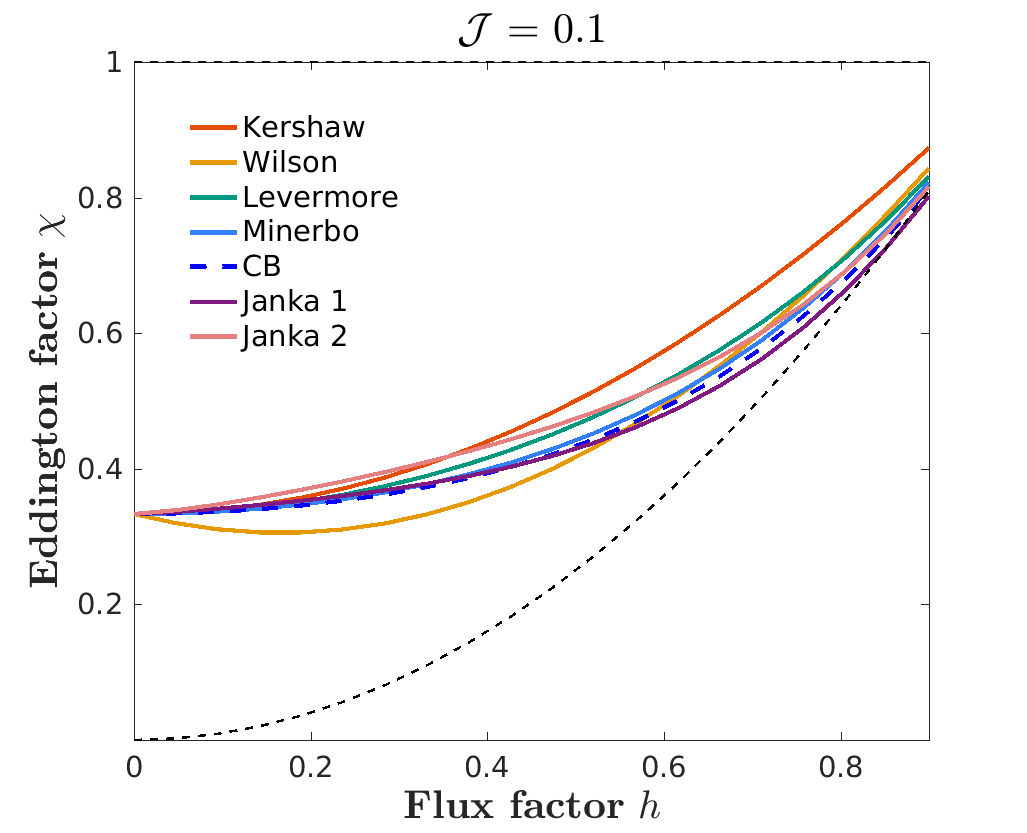
\includegraphics[width=0.5\textwidth]{figures/Closures0_10}
    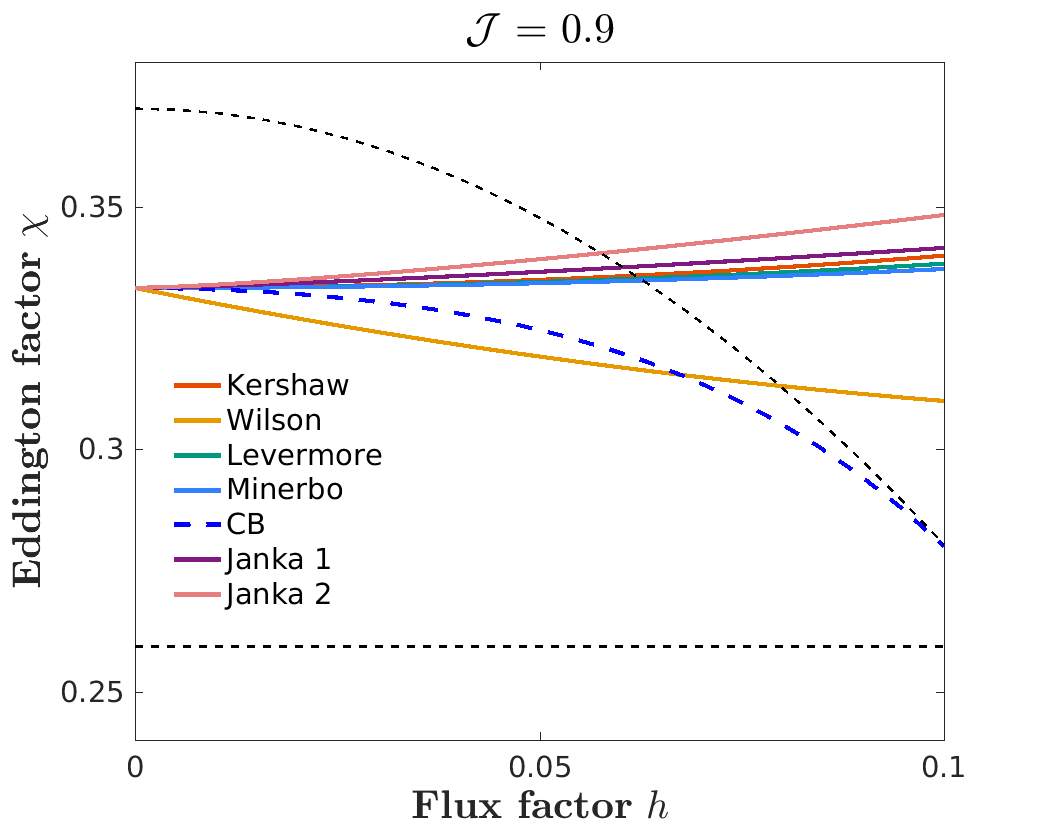
\includegraphics[width=0.5\textwidth]{figures/Closures0_90}
  \end{tabular}
   \caption{Plot of Eddington factors $\chi$ versus flux factor $h$ for different values of $\cJ$ for various algebraic closures: $\cJ=0.1$ (left panel, low occupancy) and $\cJ=0.9$ (right panel, high occupancy).  In each panel we plot the Eddington factors of two-moment closures due to Kershaw (red), Wilson (yellow), Levermore (green), Minerbo (light blue), Cernohorsky \& Bludman (blue), Janka~1 (purple), and Janka~2 (pink) .  We also plot $\chi_{\mbox{\tiny min}}$ and $\chi_{\mbox{\tiny max}}$, defined in Eq.~\eqref{eq:eddingtonFactorBounds} (lower and upper dashed black lines, respectively).}
  \label{fig:EddingtonFactorsWithDifferentClosure}
\end{figure}
\section{Spatial Discretization}\label{se:SpatialDiscretization}

We discretize the two-moment model with a simple first-order finite volume method to illustrate how the closure affects the realizability-preserving property of the method.  
By assuming that the moments at time level $t^{n}$ ($\bcM^{n}$) satisfy the bounds in Eq.~\eqref{eq:MomentsBounds}, our goal is to identify sufficient conditions such that the moments at time level $t^{n+1}$ ($\bcM^{n+1}$) also satisfy the bounds.
To simplify, we limit the discussion to one spatial dimension and employ a uniform Cartesian mesh.  
(The extension to multiple spatial dimensions and high-order discretization using the discontinuous Galerkin method is given in~\cite{chu_etal_2018}.)

We divide the spatial domain $D$ into $N$ uniform cells and denote the $i$-th cell by $\bK_{i}$, with $i = 1,\ldots,N$; i.e.,
\begin{equation*}
  D = \cup_{i = 1}^{N} \bK_{i} \quad \text{with} \quad
  \bK_{i}=\{\,x : x\in(x_{i-1/2}, x_{i+1/2})\},
\end{equation*}
and cell width $\dx = D/N$.  
The cell-average of the moments is defined as
\begin{equation}
  \bcM_{i} = \dfrac{1}{\dx} \int_{\bK_i}\bcM dx.
\end{equation}
Integrating Eq.~\eqref{eq:momentEquations} over each cell $\bK_{i}$ gives
\begin{equation}
  \dfrac{d \bcM_{i}}{d t} = - \dfrac{1}{\dx} \left( \widehat{\bcF}(\bcM_{i},\bcM_{i+1}) -  \widehat{\bcF}(\bcM_{i-1},\bcM_{i})\right) + \f{1}{\tau}\,\cC(\bcM_{i}),
  \label{eq:SemiDiscretizatedMomentEquation}
\end{equation}
where $\widehat{\bcF}(\vect{\cM}_{a},\vect{\cM}_{b})$ is the numerical flux and $\f{1}{\tau}\,\cC(\bcM_{i})$ is the collision term evaluated with $\bcM_{i}$.
In this paper we use the global Lax-Friedrichs flux (setting the largest absolute eigenvalue of the flux Jacobian to one):
\begin{equation}
  \widehat{\bcF}_{\LF}(\vect{\cM}_{a},\vect{\cM}_{b})
  =\f{1}{2}\,\big(\,\bcF(\vect{\cM}_{a})+\bcF(\vect{\cM}_{b})-(\,\vect{\cM}_{b}-\vect{\cM}_{a}\,)\,\big).
  \label{eq:Lax-Friedrichs flux}
\end{equation}
By treating the transport term explicitly with forward Euler and the collision term implicitly with backward Euler, we have
\begin{align}
  \bcM_{i}^{n+1} = \widetilde{\bcM}^{n}_{i} + \f{\dt}{\tau}\,\cC(\bcM^{n+1}_{i}),
  \label{eq:MomentIMEX}
\end{align}
where we have defined
\begin{align}
  \widetilde{\bcM}^{n}_{i} 
  & = \bcM_{i}^{n} - \frac{\dt}{\dx} \left( \widehat{\bcF}_{\LF}(\bcM^{n}_{i},\bcM^{n}_{i+1}) -  \widehat{\bcF}_{\LF}(\bcM^{n}_{i-1},\bcM^{n}_{i})\right)\nonumber \\
  & = (1-\beta)\bcM_{i}^{n} + \beta\left[ \f{1}{2}\left( \bcM^{n}_{i+1}-\bcF(\bcM^{n}_{i+1})\right)  + \f{1}{2}\left( \bcM^{n}_{i-1}+\bcF(\bcM^{n}_{i-1})\right)\right],
  \quad\beta = \frac{\dt}{\dx}.  
\label{eq:widetildeM}
\end{align}

Considering Eqs.~\eqref{eq:MomentIMEX} and \eqref{eq:widetildeM} and assuming that $\bcM_{i}^{n}$ is realizable for all $i$, it can be shown (Lemma~3 in~\cite{chu_etal_2018}) that $\bcM^{n+1}_{i}$ is realizable provided $\f{\dt}{\tau} > 0$. 
%and $\widetilde{\bcM}^{n}_{i}$ is realizable.  
In Eq.~\eqref{eq:widetildeM}, if $\beta \in [0,1]$, $\widetilde{\bcM}^{n}_{i}$ is expressed as a convex combination of $\bcM_{i}^{n}$ and the expression in the square brackets on the right-hand side of Eq.~\eqref{eq:widetildeM}.  
It follows that $\widetilde{\bcM}^{n}_{i}$ is realizable if the expression inside the square brackets is realizable.  
It can be shown (Lemma~2 in~\cite{chu_etal_2018}) that the expression in square brackets is realizable for a distribution satisfying $f\in[0,1]$.  
For the two-moment model considered here, realizability depends on the algebraic closure.  
Specifically, if $\bcM_{i}^{n}$ is realizable and the Eddington factor satisfies the bounds in Eq.~\eqref{eq:eddingtonFactorBounds}, then $\bcM^{n+1}_{i}$ is realizable provided $\beta \in [0,1]$.  
Thus, realizability of $\bcM^{n+1}_{i}$ requires both a closure based on Fermi-Dirac statistics and a Courant-Friedrichs-Lewy (CFL) condition $\dt\le\dx$.  
\section{Time Integration} \label{se:TimeIntegration}

Suppose that an algebraic closure based on Fermi-Dirac statistics is used (i.e., the Eddington factor satisfies Eq.~\eqref{eq:eddingtonFactorBounds}).
Here we consider the construction of an Implicit-Explicit (IMEX) time integration scheme that maintains the bounds in Eq.~\eqref{eq:MomentsBounds}.  
The semi-discretization of the two-moment model results in a system of ordinary differential equations of the form
\begin{equation}
  \dot{\vect{u}} = \vect{\cT}(\vect{u}) + \vect{\cQ}(\vect{u}),
\end{equation}
where the solution vector
\begin{equation}
  \vect{u}(t) = \left( \bcM_{1}(t),\ldots,\bcM_{N}(t)\right) ^{T}
\end{equation}
is the collection of all cell-averaged moments, $\vect{\cT}$ is the transport operator, corresponding to the first term on the right-hand side of Eq.~\eqref{eq:SemiDiscretizatedMomentEquation}, and $\vect{\cQ}$ is the collision operator, corresponding to the second term on the right-hand side of Eq.~\eqref{eq:SemiDiscretizatedMomentEquation}.  

Since the set of realizable moments is convex, convex-invariant schemes, which map the initial values into this set, can be used to design realizability-preserving methods for the two-moment model.
Ideally, the scheme should also be high-order accurate and work well in the asymptotic diffusion limit (characterized by frequent collisions and long time scales).  
The following discussion considers the construction of such convex-invariant schemes.  

\subsection{Standard IMEX Schemes}

Treating the transport operator explicitly and the collision operator implicitly, a standard $s$-stage IMEX scheme takes the following form~\cite{pareschiRusso_2005}: 
\begin{align}
  \vect{u}^{(i)}
  &=\vect{u}^{n}
  +\dt\sum_{j=1}^{i-1}\tilde{a}_{ij}\,\vect{\cT}(\vect{u}^{(j)})
  +\dt\sum_{j=1}^{i}a_{ij}\,\vect{\cQ}(\vect{u}^{(j)}),
  \quad i=1,\ldots,s, \label{imexStages} \\
  \vect{u}^{n+1}
  &=\vect{u}^{n}
  +\dt\sum_{i=1}^{s}\tilde{w}_{i}\,\vect{\cT}(\vect{u}^{(i)})
  +\dt\sum_{i=1}^{s}w_{i}\,\vect{\cQ}(\vect{u}^{(i)}), \label{imexIntermediate} 
\end{align}
where $(\tilde{a}_{ij})$ and $(a_{ij})$, coefficients of the $i$-th stage, are elements of matrices $\tilde{A}$ and $A$, respectively.
The matrices $\tilde{A}$ and $A$ are lower triangular.
($\tilde{A}$ is strictly lower triangular so that the transport part is explicit.)  
The vectors $\tilde{\vect{w}}=(\tilde{w}_{1},\ldots,\tilde{w}_{s})^{T}$ and $\vect{w}=(w_{1},\ldots,w_{s})^{T}$ are the weights in the assembly step in Eq.~\eqref{imexIntermediate}.
These coefficients and weights must satisfy certain order conditions for consistency, accuracy, and other properties.  
For second-order temporal accuracy, the following conditions are required~\cite{hairer_1981}:
\begin{equation}
  \sum_{i=1}^{s}\tilde{w}_{i}=\sum_{i=1}^{s}w_{i}=1,
  \label{orderConditions1}
\end{equation}
and
\begin{equation}
  \sum_{i=1}^{s}\tilde{w}_{i}\,\tilde{c}_{i}
  =\sum_{i=1}^{s}\tilde{w}_{i}\,c_{i}
  =\sum_{i=1}^{s}w_{i}\,\tilde{c}_{i}
  =\sum_{i=1}^{s}w_{i}\,c_{i}=\f{1}{2}, 
  \label{orderConditions2}
\end{equation}
where $\tilde{c}_{i} = \sum_{j=1}^{s}\tilde{a}_{ij}$ and $c_{i}=\sum_{j=1}^{s}a_{ij}$.

The IMEX scheme is called globally stiffly accurate (GSA) if the coefficients satisfy~\cite{dimarcoPareschi2013}:
\begin{equation}
  a_{si}=w_{i} \quad\text{and}\quad \tilde{a}_{si}=\tilde{w}_{i}, \quad \text{for} \quad i=1,\ldots,s.
\end{equation}
Then, $\vect{u}^{n+1} = \vect{u}^{(s)}$, which is simplifying because the assembly step in Eq.~\eqref{imexIntermediate} is omitted.  
IMEX schemes are further classified by the structure of the implicit matrix $A$.  
If $A$ is invertible, the IMEX scheme is of type~A~\cite{pareschiRusso_2005}.  
If $a_{i1} = 0$ for $i=1,\ldots,s$, $w_{1} = 0$, and the submatrix consisting of the last $s-1$ rows and columns is invertible, the IMEX scheme is of type~ARS~\cite{ascher_etal_1997,pareschiRusso_2005}.  

\subsection{Convex-Invariant IMEX Schemes}

To be convex-invariant, the coefficients and weights defining the IMEX scheme must satisfy additional constraints.
Our goal is to find constraints on $a_{ij}$, $\tilde{a}_{ij}$, $\tilde{w}_{i}$, and $w_{i}$ that enable each $\vect{u}^{(i)}$ in Eq.~\eqref{imexStages} to be expressed as a convex combination of realizable states.  
Following Hu et al.~\cite{hu_etal_2018}, the stage values in Eq.~\eqref{imexStages} can be rewritten as
\begin{equation}
  \vect{u}^{(i)}
  =\sum_{j=0}^{i-1}c_{ij}\Big[\,\vect{u}^{(j)}+\hat{c}_{ij}\,\dt\,\vect{\cT}(\vect{u}^{(j)})\,\Big] + a_{ii}\,\dt\,\vect{\cQ}(\vect{u}^{(i)}),\quad i=1,\ldots,s,
  \label{eq:imexStagesRewrite}
\end{equation}
where $c_{ij}$ and $\hat{c}_{ij}\equiv\tilde{c}_{ij}/c_{ij}$ are defined in terms of $a_{ij}$ and $\tilde{a}_{ij}$.
For IMEX schemes of type~ARS, $c_{ij}$ and $\tilde{c}_{ij}$ are given by~\cite{hu_etal_2018}
    \begin{equation}
     \begin{aligned}
      c_{i0} &= 1-\sum_{j=2}^{i-1}\sum_{l=j}^{i-1}a_{il}b_{lj}, \quad &
      c_{ij} &= \sum_{l=j}^{i-1}a_{il}b_{lj}, \\
      \tilde{c}_{i0} &= \tilde{a}_{i1}+\sum_{j=2}^{i-1}a_{ij}\tilde{b}_{j1}, \quad &
      \tilde{c}_{ij} &= \tilde{a}_{ij}+\sum_{l=j+1}^{i-1}a_{il}\tilde{b}_{lj},  
     \end{aligned}
     \label{eq:positivityCoefficientsARS}
    \end{equation}
    \begin{equation}
      b_{ii} = \f{1}{a_{ii}}, \quad
      b_{ij} = -\f{1}{a_{ii}}\sum_{l=j}^{i-1}a_{il}b_{lj}, \quad
      \tilde{b}_{ij} = -\f{1}{a_{ii}}\Big(\tilde{a}_{ij}+\sum_{l=j+1}^{i-1}a_{il}\tilde{b}_{lj}\Big).  
    \end{equation}
Note that $c_{i1}=\tilde{c}_{i1}=0$ in Eq.~\eqref{eq:positivityCoefficientsARS}, so that $\sum_{j=0}^{i-1}c_{ij}=1$.

If the IMEX scheme is GSA, $\vect{u}^{n+1} = \vect{u}^{(s)}$.  
Moreover, if $c_{ij},\tilde{c}_{ij}\ge0$ and $a_{ii}>0$, each stage in Eq.~\eqref{eq:imexStagesRewrite} is a convex combination of explicit Euler steps (with time step $\hat{c}_{ij}\dt$), followed by an implicit Euler step.  
Each of the explicit Euler steps has a time step condition that ensures its realizability given by $\hat{c}_{ij}\,\dt\leq\dx$; the CFL condition of the scheme.
Using results proved in~\cite{chu_etal_2018} and discussed in Section~\ref{se:SpatialDiscretization}, the IMEX scheme is convex-invariant and realizability-preserving for the two-moment model in Section~\ref{se:SpatialDiscretization} provided
\begin{equation}
  \max(\hat{c}_{ij})\,\dt \leq \dx.  
\end{equation}
(This CFL condition becomes more restrictive with high-order DG spatial discretization~\cite{chu_etal_2018}.)

\subsection{Diffusion Accurate, Convex-Invariant IMEX Schemes}

Accuracy in the diffusion limit is another important property to consider when an IMEX scheme is applied to the two-moment model.  
In the diffusion limit, the distribution function is nearly isotropic, so $\vect{\cK}\approx\f{1}{3}\,\cJ\,\vect{I}$ and $\vect{\cH}\approx-\f{1}{3}\,\tau\,\nabla\cJ$, and the two-moment model is approximately governed by (e.g., \cite{jinLevermore_1996})
\begin{equation}
  \pd{\cJ}{t} + \nabla\cdot\vect{\cH} = 0
  \quad\text{and}\quad
  \vect{\cH} = - \tau\,\nabla\cdot\vect{\cK}.  
  \label{eq:diffusionLimit}
\end{equation}
In the context of IMEX schemes, the above relationships imply that the following relations should hold~\cite{chu_etal_2018}:
\begin{equation}
   \vect{e}_{i}^{T}A^{-1}\tilde{A}\,\vect{e} = 1, \quad i=1,\ldots,s,
   \label{diffusionAccuracy}
\end{equation}
where $\vect{e}_{i}$ is the $i$th column of the $s\times s$ identity matrix, $\vect{e}$ is the vector of ones, and $A$ and $\tilde{A}$ are the matrices of the coefficients $(\tilde{a}_{ij})$ and $(a_{ij})$.
Eq.~\eqref{diffusionAccuracy} implies:
\begin{equation}
  c_{i} = \tilde{c}_{i}, \quad i=1,\ldots,s.
\end{equation}
We have proved in \cite{chu_etal_2018} that only IMEX schemes of type~ARS can be both diffusion accurate and convex-invariant.  
(Another short proof follows from the fact that IMEX schemes of type~A have $\tilde{c}_1 = 0$ while $c_i \neq 0$.)  

\subsection{PD-ARS IMEX schemes}

Unfortunately, coefficients satisfying the order conditions in Eqs.~\eqref{orderConditions1}-\eqref{orderConditions2} and the conditions for convex-invariance do not exist for the standard IMEX scheme in Eqs.~\eqref{imexStages}-\eqref{imexIntermediate}, unless a small time step is invoked that makes the scheme essentially explicit.  
To circumvent this problem, correction steps can be introduced after the assembly step in Eq.~\eqref{imexIntermediate} (e.g., \cite{chertock_etal_2015,hu_etal_2018}).  
However, the correction steps can impose time step constraints for realizability or accuracy in the diffusion limit that ruin the efficiency gains expected from the IMEX scheme.  
Because of this, we sacrifice overall high-order accuracy, and aim for IMEX schemes that are high-order accurate in the streaming limit, diffusion accurate, and convex-invariant.  
Combining these requirements we seek GSA IMEX schemes of type~ARS with coefficients satisfying the following constraints~\cite{hu_etal_2018,chu_etal_2018}:
\begin{enumerate}
    \item Consistency of the implicit coefficients:
    \begin{equation}
      \sum_{i=1}^{s}w_{i}=1.
    \end{equation}
    \item High-order accuracy in the streaming limit.
    For second-order accuracy:
    \begin{equation}
      \sum_{i=1}^{s}\tilde{w}_{i}=1
      \quad\text{and}\quad
      \sum_{i=1}^{s}\tilde{w}_{i}\,\tilde{c}_{i}=\f{1}{2}.
      \label{eq:orderConditionsEx}
    \end{equation}
    For third-order accuracy: 
    \begin{equation}
    \sum_{i=1}^{s}\tilde{w}_{i}=1,
          \quad
          \sum_{i=1}^{s}\tilde{w}_{i}\,\tilde{c}_{i}=\f{1}{2},
          \quad
          \sum_{i=1}^{s}\tilde{w}_{i}\,\tilde{c_{i}}^2 = \f{1}{3}
          \quad\text{and}\quad
          \sum_{i=1}^{s}\tilde{w}_{i}\,\tilde{a_{ij}}\tilde{c}_{j}= \f{1}{6}.
    \end{equation}
    \item Diffusion accuracy:
    \begin{equation}
      c_{i}=\tilde{c}_{i}, \quad i=1,\ldots,s.
      \label{eq:diffusionCondition}
    \end{equation}
    \item Convex-invariance:
    \begin{align}
      &a_{ii}>0, \quad c_{i0},\tilde{c}_{i0}\ge0, \quad \text{for} \quad i=2,\ldots,s, \nonumber \\
      &\text{and} \quad c_{ij},\tilde{c}_{ij}\ge0, \quad \text{for} \quad i=3,\ldots,s, \quad\text{and}\quad j=2,\ldots,i-1,
      \label{eq:convexInvariant}
    \end{align}
    with $\sum_{j=0}^{i-1}c_{ij}=1$, for $i=1,\ldots,s$, and $c_{\Sch}:=\min_{\substack{i = 2,\ldots,s \\ 
                  j = 0,2,\ldots,i-1}}\,\f{1}{\hat{c}_{ij}}>0$.
                  
    (Note that the greater the $c_{\Sch}$, the larger the time step can be.
    And $c_{\Sch} \leq 1$.)
    \item Having less than five stages ($s\le4$)\label{cod:statges}.
    \item Are globally stiffly accurate: $a_{si}=w_{i}$ and $\tilde{a}_{si}=\tilde{w}_{i},\quad i=1,\ldots,s$. 
\end{enumerate}
Fortunately, these IMEX schemes are easy to find.  
(The constraint in \eqref{cod:statges} is introduced from efficiency considerations to limit the number of implicit solves.)
We call the IMEX schemes satisfying the above conditions {PD-ARS} (see also Definition~3 in~\cite{chu_etal_2018}), and we provide two optimal PD-ARS schemes below: PD-ARS2 and PD-ARS3, each limiting to the optimal second-order and third-order SSPRK schemes from~\cite{shuOsher_1988}, respectively.
\subsubsection{PD-ARS2}

The optimal 3-stage PD-ARS, PD-ARS2, in the standard double Butcher tableau form, with explicit tableau ($\tilde{A}$) on the left and implicit tableau ($A$) on the right, is given by
\begin{align}
  &\begin{array}{c | c c c}
  	0 & 0   & 0 & 0 \\
  	1 & 1   & 0 & 0 \\
  	1 & 1/2 & 1/2 & 0 \\ \hline
  	  & 1/2 & 1/2 & 0 
  \end{array}
  \qquad
  \begin{array}{c | c c c}
  	0 & 0 & 0            & 0            \\
  	1 & 0 & 1            & 0            \\
  	1 & 0 & 1/2 & 1/2 \\ \hline
  	  & 0 & 1/2 & 1/2
  \end{array}
\end{align}
Note its explicit tableau is SSPRK2. 
For this scheme, only two implicit solves are needed per time step and $c_{\Sch}= 1$, which implies that the time step restriction for preserving moment realizability is only due to the explicit part.  

\subsubsection{PD-ARS3}

The optimal 4-stage PD-ARS, PD-ARS3, is given in its standard double Butcher tableau form (explicit tableau on the left and implicit tableau on the right) by
\begin{align}
  &\begin{array}{c | c c c c}
  	    &     &     &     &  \\
  	 1  & 1   &     &     &  \\
  	1/2 & 1/4 & 1/4 &  \\
  	 1  & 1/6 & 1/6 & 2/3 &  \\ \hline
  	    & 1/6 & 1/6 & 2/3 &
  \end{array}
  \qquad
  \begin{array}{c | c c c c}
  	0 & 0 & 0            & 0            \\
  	1 & 0 & 1            & 0            \\
  	1/2 & 0 & 1/4 & 1/4 \\ 
  	1 & 0 & 1/6 & 1/6 & 2/3\\\hline
  	  & 0 & 1/6 & 1/6 & 2/3
  \end{array}
\end{align}
Its explicit tableau is SSPRK3. 
This scheme requires three implicit solves per time step, and $c_{\Sch}= 1$.  
Since PD-ARS3 is not more accurate than PD-ARS2 in collision-dominated regions (see our results in Section~\ref{se:NumericalTests}), it may not offer any practical advantage over PD-ARS2.  

\section{Numerical Tests}\label{se:NumericalTests}

In this section we present numerical results obtained with the PD-ARS schemes in Section~\ref{se:TimeIntegration}.
The tests in Section \ref{se: Accuracy Tests} are designed to compare the accuracy of the schemes in streaming, absorption, and scattering-dominated regimes in one spatial dimension.
The test in Section \ref{se: Neutrino Stationary State Test} demonstrates the convex-invariance of PD-ARS schemes.
All the tests in this section were computed with third-order accurate spatial discretization (polynomials of degree $k=2$) and time step $\dt = 0.1 \times \dx $, using the DG scheme from~\cite{chu_etal_2018}.

\subsection{Accuracy Tests}
\label{se: Accuracy Tests}

To compare the accuracy of the IMEX schemes, we applied our PD-ARS schemes and the SSP2332 scheme from Pareschi \& Russo~\cite{pareschiRusso_2005} to problems with known smooth solutions in streaming, absorption (damping), and scattering-dominated (diffusing) regimes in one spatial dimension.
All the tests in this subsection were computed with the maximum entropy closure in the low-occupancy limit (i.e., the Minerbo closure).  
In the streaming test, the second- and third-order accurate explicit strong-stability-preserving Runge-Kutta methods from~\cite{gottlieb_etal_2001} (SSPRK2 and SSPRK3, respectively) are also included.  
To compare the numerical results to analytic solutions, the averaged absolute error or the averaged relative error are computed in the $L^{1}$-error norm.
We compute the absolute error for the streaming and diffusion tests and the relative error for the damping test.
They are averaged over the cell with an equal-weight quadrature for the cell integrals.
To examine the convergence, we let the number of elements ($N$) vary from 8 to 128.  

\subsubsection{Sine Wave Streaming}

The sine wave streaming test is designed to test accuracy in the free-steaming regime; i.e. $\sigma_{\Ab} = \sigma_{\Scatt} = 0$.
A periodic domain of unit length is used and the initial condition is $\cJ_{0} = \bcH_{0} = 0.5+0.49\times\sin\big(2\pi\,x\big)$.
We evolve the test until the sine wave has completed 10 crossings of the domain.
Figure~\ref{fig: SineWaveStreaming} plots the absolute error for the number density versus the number of elements $N$.
We see the errors obtained with SSPRK3 and PD-ARS3 are smallest and decrease as $N^{-3}$, as expected for a scheme combining third-order accurate time stepping with third-order accurate spatial discretization.
For all the other schemes, using second-order accurate explicit time stepping, the error decreases as $N^{-2}$.
Among the second-order schemes, SSP2332 has the smallest error.
In the streaming limit, the PD-ARS schemes reduce to SSPRK schemes --- PD-ARS2 to SSPRK2 and PD-ARS3 to SSPRK3, respectively.
Therefore, the absolute errors of PD-ARS schemes and SSPRK schemes are indistinguishable.  

\begin{figure}[h]
  \centering
    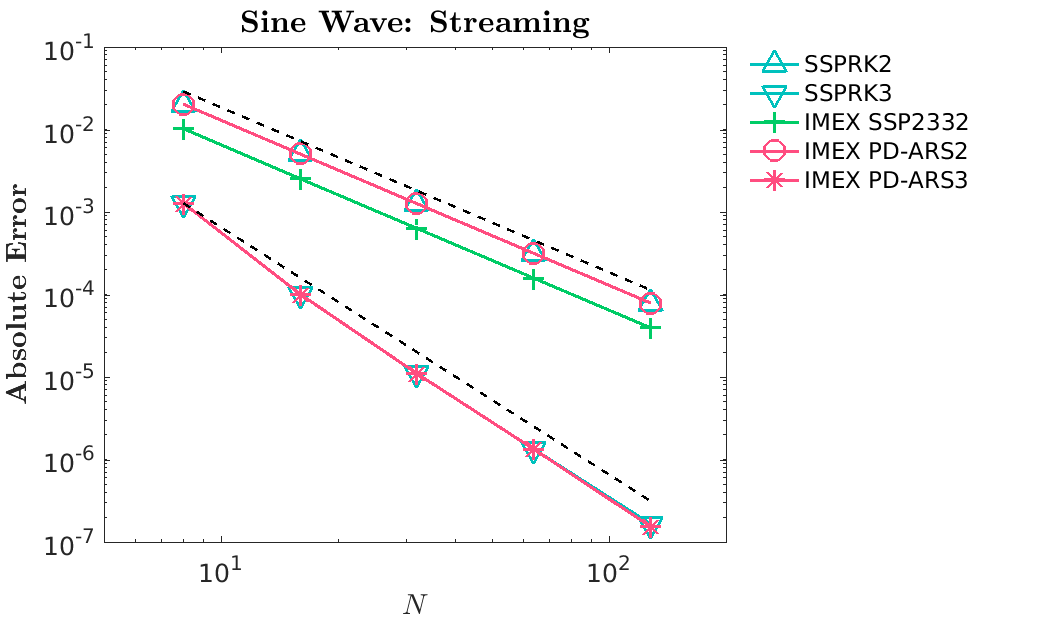
\includegraphics[width=0.8\textwidth]{figures/SineWaveStreaming}
   \caption{Absolute error versus number of elements, $N$, for the streaming sine wave test.  Results employing various time stepping schemes are compared: SSPRK2 (cyan triangles pointing up), SSPRK3 (cyan triangles pointing down), SSP2332 (green crosses), PD-ARS2 (light red circles) and PD-ARS3 (light red asterisks). Black dashed reference lines are proportional to $N^{-2}$ (top), and $N^{-3}$ (bottom), respectively.}
   \label{fig: SineWaveStreaming}
\end{figure}

\subsubsection{Sine Wave Damping}

The next test, adapted from~\cite{skinnerOstriker_2013}, is designed for absorption-dominated regimes, with $\sigma_{\Scatt} = 0$ and $f_0 = 0$, which results in exponential damping of the wave amplitude.
A periodic domain $D=\{x:x\in[0,1]\}$ and initial condition $\cJ_{0} = \bcH_{0} = 0.5+0.49\times\sin\big(2\pi\,x\big)$ are used.
The amplitude of the analytical solution decreases as $e^{-\sigma_{\Ab} t}$.
For $\sigma_{\Ab}$ = 0.1, 1 and 10 we evolve the test until the initial condition has been damped by a factor $e^{-10}$. 
Figure~\ref{fig:SineWaveDamping} shows convergence results of the test in the relative error.
Results for $\sigma_{\Ab}=0.1$, $1$, and $10$ are plotted with red, green, and blue lines, respectively.
SSP2332 is the most accurate among these schemes for $\sigma_{\Ab}= 1$ and 10. 
For $\sigma_{\Ab}=0.1$, PD-ARS2 is the most accurate scheme for $N=8$ and $N=16$. 
We have seen the same behavior for the scheme proposed by McClarren et al.~\cite{mcclarren_etal_2008} (PC2 in~\cite{chu_etal_2018}).
Since these are special cases for $N=8$ and $N=16$, we do not recommend PD-ARS2 instead of SSP2332 for the damping problem.
Only SSP2332, a second-order accurate scheme, displays a second-order convergence rate.  
The PD-ARS schemes are first-order accurate.

\begin{figure}[h]
  \centering
    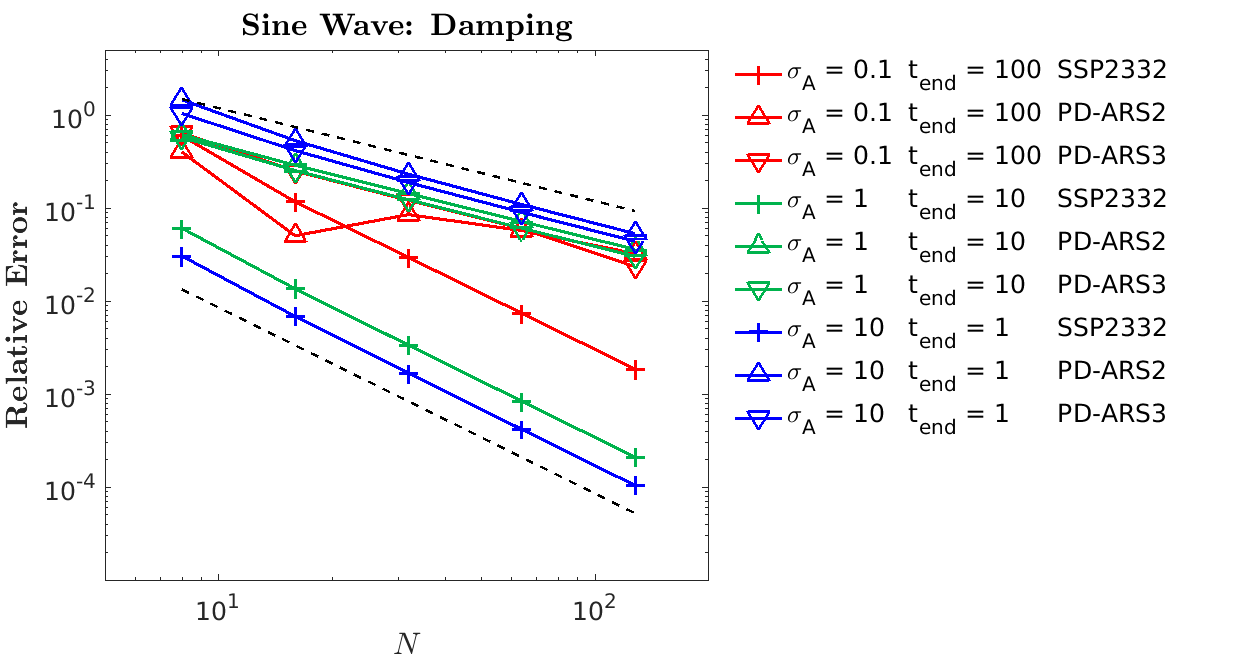
\includegraphics[width=0.9\textwidth]{figures/SineWaveDamping}
   \caption{Relative error versus number of elements, $N$, for the damping sine wave test. Results for different values of the absorption opacity $\sigma_{\Ab}$, employing various IMEX time stepping schemes, are compared.  Errors for $\sigma_{\Ab}=0.1$, $1$, and $10$ are plotted with red, green, and blue lines, respectively.  The IMEX schemes employed are SSP2332 ($+$), PD-ARS2 (triangles pointing up) and PD-ARS3 (triangles pointing down).  Black dashed reference lines are proportional to $N^{-1}$ (top) and $N^{-2}$ (bottom), respectively.}
  \label{fig:SineWaveDamping}
\end{figure}

\subsubsection{Sine Wave Diffusion}

The final test with known smooth solutions, adopted from~\cite{radice_etal_2013}, is the sine wave diffusion test; i.e. $\sigma_{\Ab} = 0$ and $f_0 = 0$.
A periodic domain $D=\{x:x\in[-3,3]\}$ with initial conditions $\cJ_{0} = 0.5+0.49\times\sin\big(\f{\pi\,x}{3}\big)$ and $\cH_{0} =-\f{1}{3\sigma_{\Scatt}}\pderiv{\cJ_{0}}{x}$ are used.  
The reference diffusion solution is given by $\cJ = \cJ_{0} \times \exp\big(-\f{\pi^2 t}{27\sigma_{\Scatt}}\big)$ and $\cH = (3\,\sigma_{\Scatt})^{-1}\pd{\cJ}{x}$.  
We evolve with $\sigma_{\Scatt}=10^{2}$, $10^{3}$, and $10^{4}$, and adjust the end time so that $t_{\mbox{\tiny end}}/\sigma_{\Scatt}=1$, 
at which time the amplitude of the sine wave has been reduced by a factor $e^{-\pi^{2}/27}\approx0.694$ for all values of $\sigma_{\Scatt}$. 
Figure~\ref{fig:SineWaveDiffusionJ} shows the absolute error, obtained using different values of $\sigma_{\Scatt}$, for various IMEX schemes at $t=t_{\mbox{\tiny end}}$, versus $N$. 
Results for $\sigma_{\Scatt}=10^{2}$, $10^{3}$, and $10^{4}$ are plotted with red, green, and blue lines, respectively.
SSP2332 and PD-ARS schemes display third-order accuracy for the number density, $\cJ$, and second-order accuracy for $\cH_{x}$, and their errors are difficult to distinguish.
For $\sigma=10^{2}$, the errors in the number density $\cJ$ do not drop below $10^{-6}$ because of differences between the two-moment model and the diffusion equation used to obtain the analytic solution.
For larger values of the scattering opacity, $\sigma=10^{3}$ or $10^{4}$, the two-moment model agrees better with the diffusion model, and we observe convergence over the entire range of $N$.
PD-ARS2 behaves as well as SSP2332 in the diffusion region but requires 33\% less implicit solves per time step.  

\begin{figure}[h]
  \centering
  \centerline{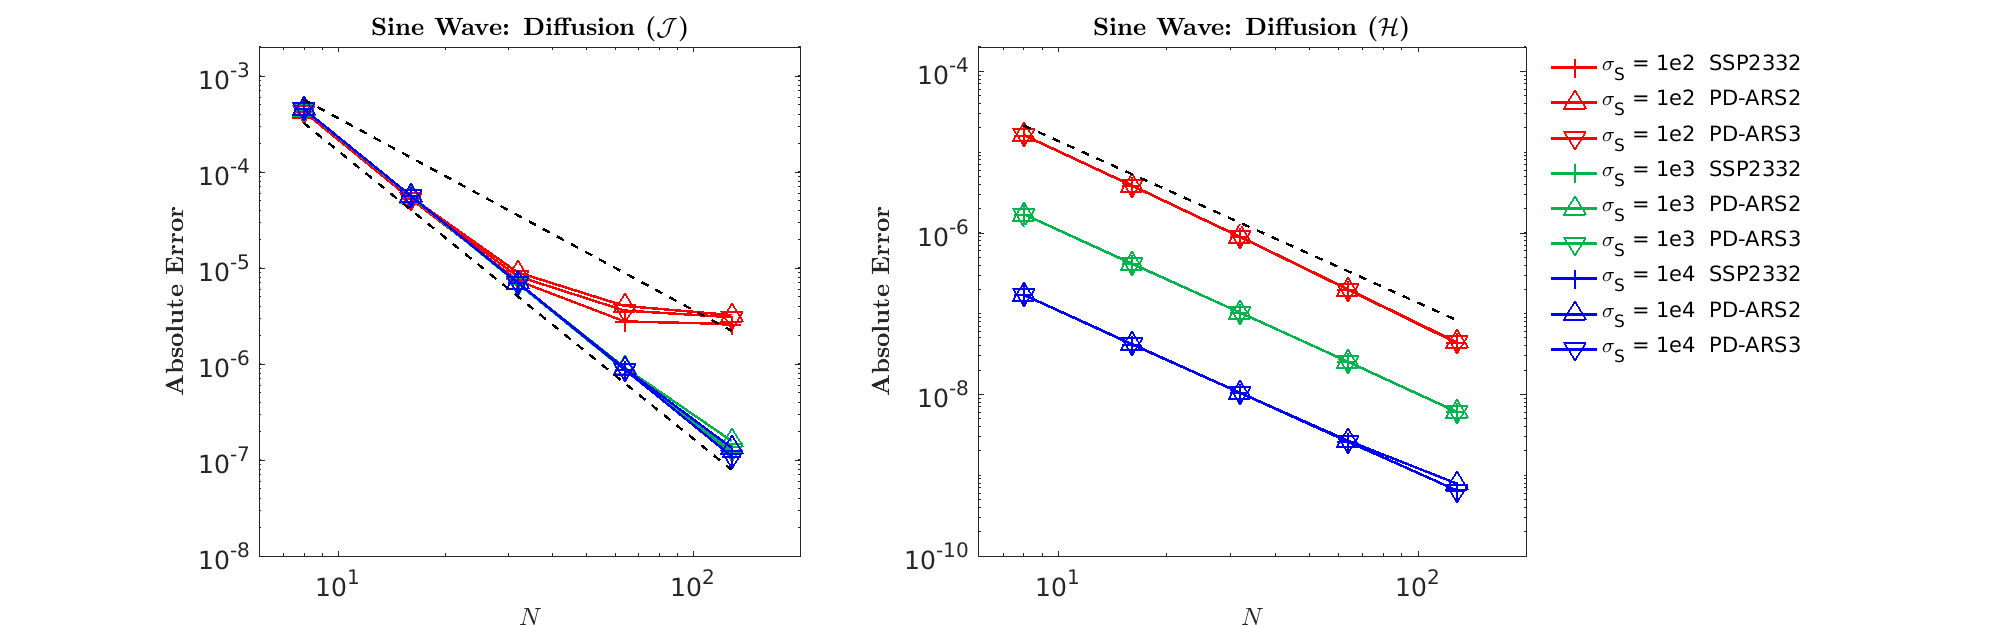
\includegraphics[width=1.2\textwidth]{figures/SineWaveDiffusion}}
   \caption{Absolute error for the number density $\cJ$ (left) and the number flux $\cH_{x}$ (right) versus number of elements for the sine wave diffusion test.  Results with different values of the scattering opacity, $\sigma_{\Scatt}$, employing different IMEX schemes, are compared.  Errors with $\sigma_{\Scatt}=10^{2}$, $10^{3}$, and $10^{4}$ are plotted with red, green, and blue lines, respectively.  The IMEX schemes employed are:  SSP2332 ($+$), PD-ARS2 (triangles pointing up), and PD-ARS3 (triangles pointing down). Black dashed lines in the left plot are reference lines proportional to $N^{-2}$ (top) and $N^{-3}$ (bottom), respectively. Black dashed line in the right plot is a reference line proportional to $N^{-2}$ .}
   \label{fig:SineWaveDiffusionJ}
\end{figure}

\subsection{Neutrino Stationary State Test} \label{se: Neutrino Stationary State Test}

In this section we consider a more ``realistic'' test: two-dimensional multigroup neutrino transport with emission, absorption, and isoenergetic scattering through a stationary background.  
\modified{This test is designed to test the realizability-preserving properties of the PD-ARS schemes.  
In the left panel in Figure~\ref{fig:NeutrinoStationaryTestEOS} we plot the thermal state of the background, which mimics a collapsed stellar core: 
\begin{subequations}
  \begin{align}
    \text{Mass Density: }~\rho & = 4 \times 10^{14} \times \dfrac{7.5}{( 7.5 + ( r / 5~\mbox{km} )^4 )} ~\text{g~cm$^{-3}$}, \\
    \text{Temperature: }~T & = 1.5 \times 10^{11} \times \dfrac{1}{1 + ( r / 50~\mbox{km} )^2 } ~\text{K}, \\
    \text{Electron Fraction: }~Y_e & = 0.25 \times \left(  1 + \dfrac{1}{1+ ( r / 50~\mbox{km} )^{-12}}  \right), 
  \end{align}
  \label{eq:NuStatinaryStateEOS}
\end{subequations}
\hspace{-6pt}where the radius $r=\sqrt{(x^{1})^{2}+(x^{2})^{2}}$ is in kilometers.  
In the right panel in Figure~\ref{fig:NeutrinoStationaryTestEOS} we plot the neutrino opacities, computed by interpolation in a pre-calculated opacity table based on~\cite{Bruenn_1985}.
This test is computed using Cartesian coordinates on a two-dimensional domain $D=\{\vect{x}\in\bbR^{2}:x^{1}\in[0,200]~\mbox{km}, x^{2}\in[0,200]~\mbox{km}\}$, using a grid of 128 elements in each direction, 10 energy groups covering $0$-$300$~MeV, reflecting inner boundaries, and outflow outer boundaries.  
Because we use Cartesian coordinates in two spatial dimensions, this problem has cylindrical geometry, and results in an artificial stratification of the radiation quantities.}
We initialize the neutrino number density to $\cJ = 10^{-99}$, the number flux density to $\bcH=0$, and evolve until an approximate steady state is reached ($t=5$~ms).
The background is kept fixed during the entire run.  
For this test, we employed both CB and Minerbo closures.  
We attempted to run this test with our PD-ARS schemes, SSP2332 from~\cite{pareschiRusso_2005}, IMEXRKCB2 proposed by Cavaglieri \& Bewley~\cite{cavaglieriBewley2015}, and the IMEX PC2 scheme proposed by McClarren et al.~\cite{mcclarren_etal_2008}.
Only the PD-ARS schemes produce realizable moments and are able to evolve to a steady state with either CB or Minerbo closure.
SSP2332 and IMEX PC2 failed after a few time steps with either CB or Minerbo closure because of the development of unrealizable moments.
Even though IMEXRKCB2 with Minerbo closure can run and reach a steady state in this test, its results are different from that of PD-ARS schemes with CB closure, and there is no guarantee of stability.  
%It's difficult to determine whether the results are in fact compromised by a particular correction step and, if so, in what way and to what degree.

Results obtained with the IMEX PD-ARS schemes are plotted in Figure~\ref{fig:NeutrinoStationaryTestEvolve} for various times: $t=0.01$~ms (top panels), 0.35~ms (middle panels), and 5.0~ms (bottom panels).  
In the left column we plot the solution in the $|\vect{\cH}|\cJ$-plane.  
In the middle column we show scatter plots of the number density $\cJ$ versus radius for select neutrino energies: 5~MeV (red lines), 16~MeV (magenta lines), and $93$~MeV (blue lines).  
In the right column we plot the flux factor $|\vect{\cH}|/\cJ$ versus radius for the same neutrino energies as in the middle column. 
In the left panels, each solution point in the domain is marked as a red dot in the $|\vect{\cH}|\cJ$-plane, and the realizable domain is shown as the light blue region.  
The figures show that all the states in the simulation with the PD-ARS schemes are realizable.
In the middle and right column, we can see how the neutrinos are generated near the core, stream out, and eventually reach an equilibrium distribution over the phase space.
\modified{The oscillations in the flux factor seen in the right columns are associated with steep gradients in the radiation field as the initial transient propagates through the computational domain.  
Note that we do not apply any limiters to prevent oscillations in the numerical solution, and these will likely go away when we implement slope limiters; e.g., as described in \cite{cockburnShu_1998}.  
The fact that we can still evolve the solution to a steady state speaks to the robustness of the scheme.}

\begin{figure}[h]
  \centering
  \begin{tabular}{cc}
    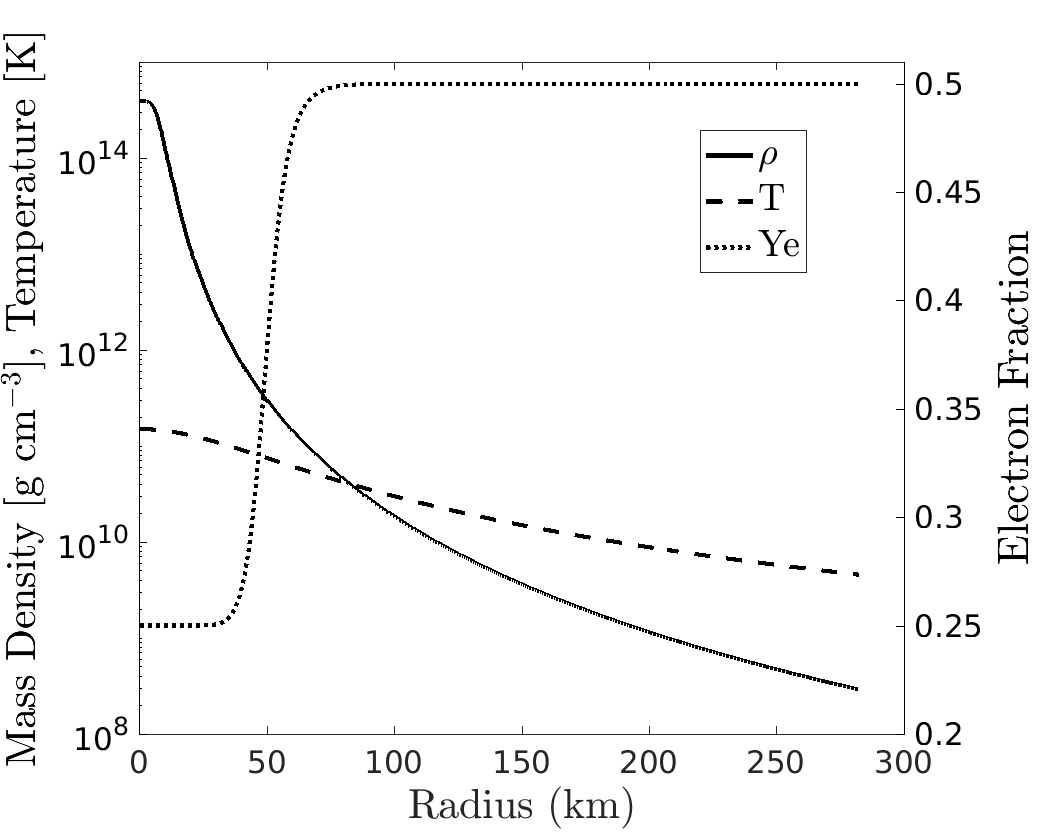
\includegraphics[width=0.45\textwidth]{figures/NStatinaryS_EOS}
    \hspace{30pt}
    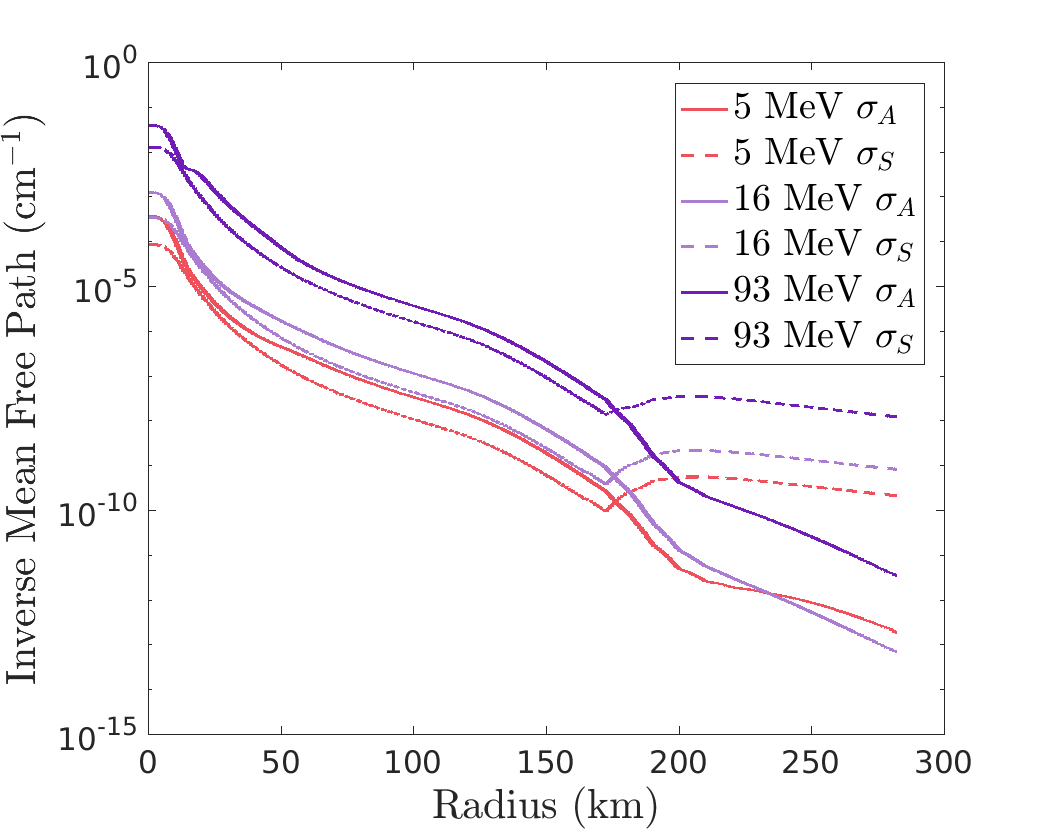
\includegraphics[width=0.45\textwidth]{figures/NSS_Opacities}
  \end{tabular}
   \caption{Left panel: thermal state of the background versus radius in the neutrino stationary state test; mass density (solid line), temperature (dashed line), and electron fraction (dotted line).  Right panel: corresponding opacities for select neutrino energies; absorptivity ($\sigma_{\Ab}$) and scattering opacity ($ \sigma_{\Scatt}$).}
   \label{fig:NeutrinoStationaryTestEOS}
\end{figure}

\begin{figure}[h]
  \centering
    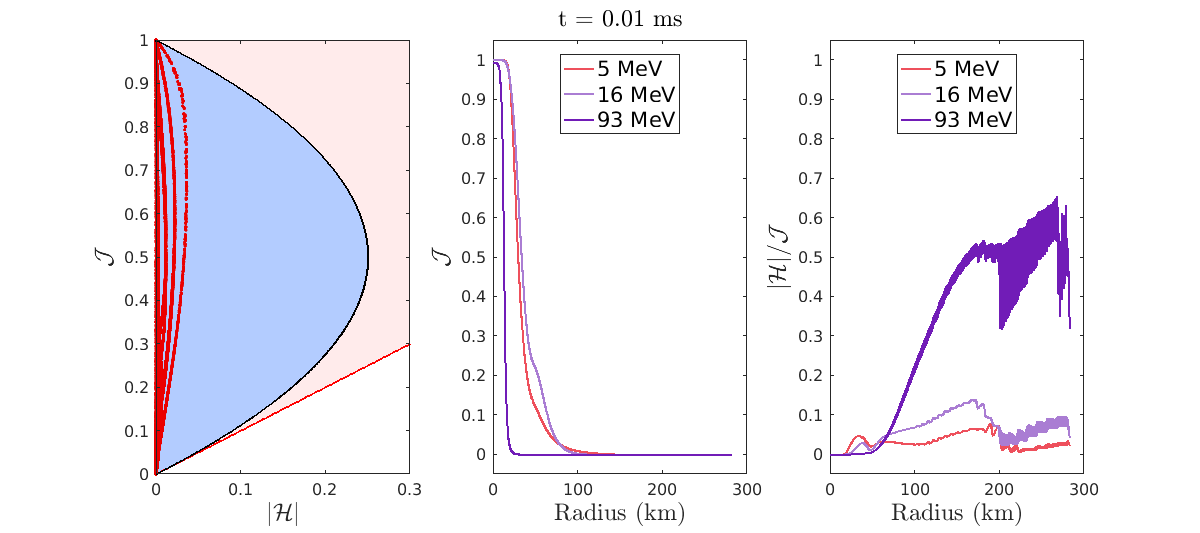
\includegraphics[width=.9\textwidth]{figures/NSS_1_1}\\
    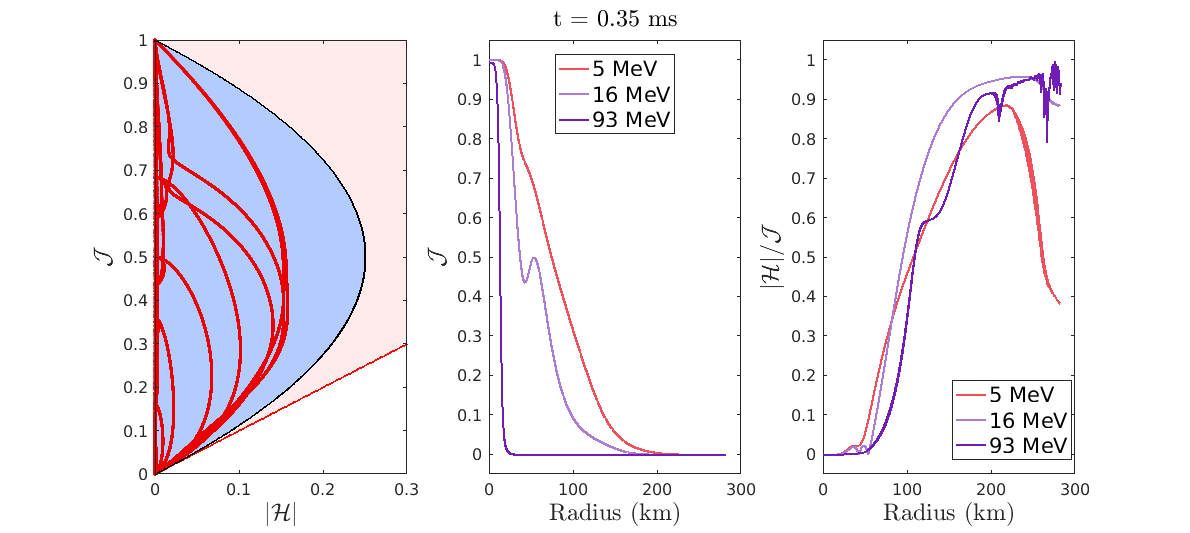
\includegraphics[width=.9\textwidth]{figures/NSS_3_1} \\
    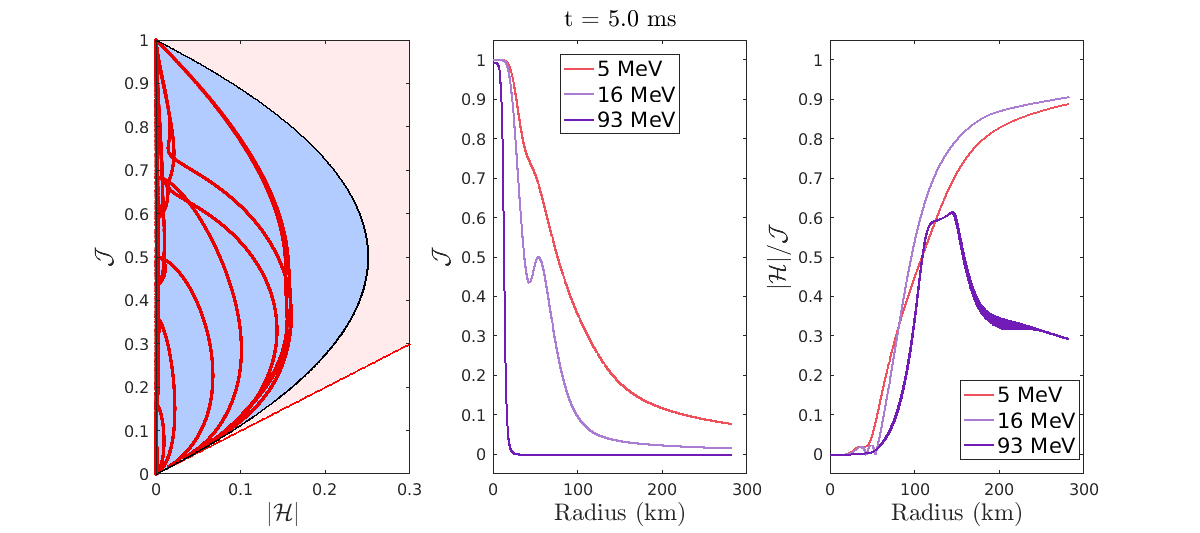
\includegraphics[width=.9\textwidth]{figures/NSS_5_1} \\
    \caption{Results from the neutrino stationary state test: moments relative to the realizable domain (left column, the light blue domain is for $f \in [0,1]$, with the black-solid-line as its boundary, while the light red domain is for $f\geq 0$, with the thin-red-solid-line as its boundary), the number density $\cJ$ versus radius (middle column), and the flux factor $|\bcH|/\cJ$ versus radius (right column), at $t = 0.01$~ms, 0.35~ms, and 5.0~ms.  For the plots in the left column, each $\bcM=(\cJ,\bcH)^{T}$ state is marked by a red dot, which are all inside the light blue region (the realizable domain for fermions).  The results of PD-ARS2 and PD-ARS3 are indistinguishable in these plots.}
    \label{fig:NeutrinoStationaryTestEvolve}
\end{figure}
\section{Summary and Outlook}\label{se:Summary}

We have developed IMEX schemes suitable for a two-moment model of neutrino transport that obey Fermi-Dirac statistics.
The scheme employs algebraic closure based on Fermi-Dirac statistics, high-order discontinuous Galerkin methods for spatial discretization, and convex-invariant time integration to maintain realizability of the moments.  
Since the realizable domain is convex and its convexity can be inherited by a convex combination, a scheme having convex combinations as its stages can preserve the realizable domain.
This encouraged us to construct realizability-preserving time integrators, realizability-preserving IMEX schemes, and a method with a realizability-preserving IMEX time integrator and high-order DG method.  

In the applications that motivate this work, the neutrino distribution function can vary from 0 to 1.  
Hence, we have considered algebraic closures based on Fermi-Dirac statistics for both low and high occupancy.  
Among the seven algebraic closures we considered -- Kershaw~\cite{kershaw_1976}, Wilson~\cite{wilson_1975,leblancWilson_1970}, Levermore~\cite{levermore_1984}, Minerbo~\cite{minerbo_1978}, Janka 1~\cite{janka_1991}, Janka 2~\cite{janka_1992}, and Cernohorsky \& Bludman~\cite{cernohorskyBludman_1994} -- only the Cernohorsky \& Bludman closure obeys Fermi-Dirac statistics for all occupancies.  
As a result, we employed the Cernohorsky \& Bludman closure for the neutrino stationary state test in Section~\ref{se: Neutrino Stationary State Test}.
We also ran our code with Minerbo closure, IMEX PC2, IMEX SSP2332 and IMEXRKCB2 schemes, and the results show that only PD-ARS schemes have stability.
In addition, closures have impact on the simulation result.
As we observed, both using PD-ARS scheme, there are $\sim30\%$ difference in the neutrino number densities (and relaxation time) between the results obtained with Minerbo closure and that with CB closure.
Even though RKCB2 with Minerbo closure luckily survived our test, the results it gave were compromised: they were closer to the results of the PD-ARS scheme with Minerbo closure than to the results of the PD-ARS scheme with CB closure.
In what way and to what degree the results are in fact compromised either by the closure or by a particular correction step for unrealizable moments are difficult to determine fully and is left for further study.


Two PD-ARS schemes are proposed.
The one with SSPRK2 has second-order accuracy while the other with SSPRK3 has third-order accuracy, and both have the strong-stability preserving property in the streaming limit.  
Their accuracy was demonstrated on problems with known smooth solutions in streaming, absorption, and scattering-dominated regimes.
The neutrino transport test with emission, absorption, and isoenergetic scattering through a stationary background, was designed to test the convex-invariance of our PD-ARS schemes. 
The neutrino stationary state test shows that a method combining an algebraic closure based on Fermi-Dirac statistics and convex-invariant time integration is promising for robust CCSN simulation.

In this work, we adopted Cartesian coordinates, a linear collision term, and a fixed material background.
More realistic problems of scientific interest, such as with energy-exchanging scattering and relativistic effects, are left for future research.
\section{Acknowledgment} \label{se:Acknowledgment}

This research is sponsored, in part, by the Laboratory Directed Research and Development Program of Oak Ridge National Laboratory (ORNL), managed by UT-Battelle, LLC for the U.S. Department of Energy under Contract No. De-AC05-00OR22725. This material is based, in part, on work supported by the U.S. Department of Energy, Office of Science, Office of Advanced Scientific Computing Research. This research was also supported by the Exascale Computing Project (17-SC-20-SC), a collaborative effort of the U.S. Department of Energy Office of Science and the National Nuclear Security Administration, and by the National Science Foundation Gravitational Physics Program (NSF-GP 1806692).

%\section*{References}
\bibliography{references/references}

\end{document}


